\documentclass[platex,a4paper,12pt,dvipdfmx]{beamer}
%\documentclass[]{beamer}
\usetheme{default}
\usepackage{tikz}
\newcommand{\maru}[2]{%
%\draw [fill=green,domain=0:360] plot ({#1+#3*cos(\x)},{#2+#3*sin(\x)});
\draw[fill=blue,thick,dotted] (#1) circle[radius=#2];
}

\begin{document}
\begin{frame}{}
  \begin{tikzpicture}
    \draw[help lines] (-5,-5) grid (5,5);
    \node (a) at  (0,5){A};
    \only<1>{\maru{-4,4}{1}\draw [->,thick](-4,4)--(a);}
    \only<2>{\maru{-3,3}{1}\draw [->,thick](-3,3)--(a);}
    \only<3>{\maru{-2,2}{1}\draw [->,thick](-2,2)--(a);}
    \only<4>{\maru{-1,1}{1}\draw [->,thick](-1,1)--(a);}
    \only<5>{\maru{0,0}{1}\draw [->,thick](-0,0)--(a);}
    \only<6>{\maru{1,1}{1}\draw [->,thick](1,1)--(a);}
    \only<7>{\maru{2,2}{1}\draw [->,thick](2,2)--(a);}
    \only<8>{\maru{3,3}{1}\draw [->,thick](3,3)--(a);}
    \only<9>{\maru{4,4}{1}\draw [->,thick](4,4)--(a);}
    \only<10>{\maru{3,3}{1}\draw [->,thick](3,3)--(a);}
    \only<11>{\maru{2,2}{1}\draw [->,thick](2,2)--(a);}
    \only<12>{\maru{1,1}{1}\draw [->,thick](1,1)--(a);}
    \only<13>{\maru{0,0}{1}\draw [->,thick](0,0)--(a);}
    \only<14>{\maru{-1,1}{1}\draw [->,thick](-1,1)--(a);}
    \only<15>{\maru{-2,2}{1}\draw [->,thick](-2,2)--(a);}
    \only<16>{\maru{-3,3}{1}\draw [->,thick](-3,3)--(a);}
    \only<17>{\maru{-4,4}{1}\draw [->,thick](-4,4)--(a);}

  \end{tikzpicture}
\end{frame}
\end{document}
